%
% loesung.tex -- Beispiel-File für die Beschreibung der Loesung
%
% (c) 2020 Prof Dr Andreas Müller, Hochschule Rapperswil
%
\section{Lösung
  \label{steps:section:loesung}}
\rhead{Lösung}
Um die bestmögliche Schrittweite zu bestimmen wird meist eine Fehlerschätzung verwendet.
Diese erhält man beispielsweise indem mann vom aktuellen Punkt aus einen Probeschritt macht.
Dabei reicht auch beim Runge-Kutta Algorithmus ein einfacher Eulerschritt aus.

\subsection{Simple Schrittweitensteuerung mit konstannter Testschrittweite
  \label{steps:subsection:simplestep}}
  Eine Möglichkeit zur Realisierung einer simplen Schrittweitensteuerung ist es, einen fixen Testschritt zu machen, 
  daraus dann eine Fehlerschätzung zu generiern, woraus sich eine der Kurve angepasste Schrittweite bestimmen lässt.
  Die Funktionsweise dieser Methode wird nun anhand der Wahrscheinlichkeitsfunktion der Standardnormalverteilung vorgeführt.
  Für die Wahrscheinlichkeitsfunktion existiert zwar keine analytische Lösung,
  doch sie lässt sich aus der Wahrscheinlichkeitdichtefunktion
  \[
    \varphi(x)=\frac{1}{\sqrt{2\pi}\sigma}\mathrm{e}^{-\frac{(x-\mu)^2}{2 \sigma}}\;|\mu=0,\sigma=1
  \]
  Berechnen:
  \[
    F(x)=\int_{-\infty}^{x} \varphi (\tilde{x}) \cdot \mathrm{d} \tilde{x}
  \]
  Damit die Funktion mittels gängiger Methoden der Differenzialrechnung analysiert werden kann,
  wird die Integralfunktion in eine Differenzialgleichung umgewandelt:
  \[
    F(x)'=\varphi(x)\;|F(-\infty)=0
  \]
  In folgendem Beispiel zur Abbildung ~\ref{buch:steps:examplessc} wurde bei $x_0=-7$ mit Startwert $F(-7)=\tilde{F}_0=0$ begonnen.
  Dabei wird für den Schritt $n$ die Steigung ($\varphi$) am Punkt $x_{n-1}, \tilde{F}_{n-1}$ (in Abbildung oranger Punkt mit rotem Kreuz) berechnet.
  Damit wird ein Eulerschritt mit der Testschrittweite $h_{test}=2$ (In Abbildung als schwarzer Balken oberhalb der x-Achse) gemacht $\implies P_{test}=(x_n+h_{test}, \tilde{F}_n+\varphi(x_n, \tilde{F}_n)$.
  Nun wird auch an diesem Punkt (In Abbildung als einsames rotes Kreuz am oberen Ende der Grafik) die Steigung ermittelt.
  Sind die beiden Steigungen ziemlich ähnlich, wird davon ausgegangen,
  dass die Kurve in diesem Bereich nur wenig ihre Richtung ändert und deshalb eine grosse Schrittweite gewählt werden darf.
  Ist der Unterschied (Abbildung, untere Grafik, Differenz zwischen phi(start), phi(test)) etwas grösser,
  wird die Schrittweite (In Abbildung roter Balken innerhalb der Testschrittweite) etwas kleiner gewählt.
  Konkret berechnet sich in diesem Beispiel die zu wählende Schrittweite wie folgt:
  \[
    h=h_{test}/|\varphi(x_n, \tilde{F}_n)-\varphi(P_{test})|/q_{factor}\; |q_{factor}=20
  \]
  Wobei die Schrittweite nach oben zusätzlich durch die Testschrittweite begrenzt wird, da der Verlauf der Kurve jenseits des Testpunktes noch nicht bekannt ist.
  Auch eine Division durch Null muss abgefangen werden, falls die Steigung in beiden Punkten identisch ist,
  wobei dann die maximale Schrittweite $h=h_{test}$ gewählt wird.
  Mit der nun ermittelten Schrittweite wird ein Runge-Kutta-Schritt (4. Ordnung) gemacht,
  wobei einer der Koeffizienten ($k_1$) bereits beim Testschritt ermittelt worden ist.

  \begin{figure}
    \centering
    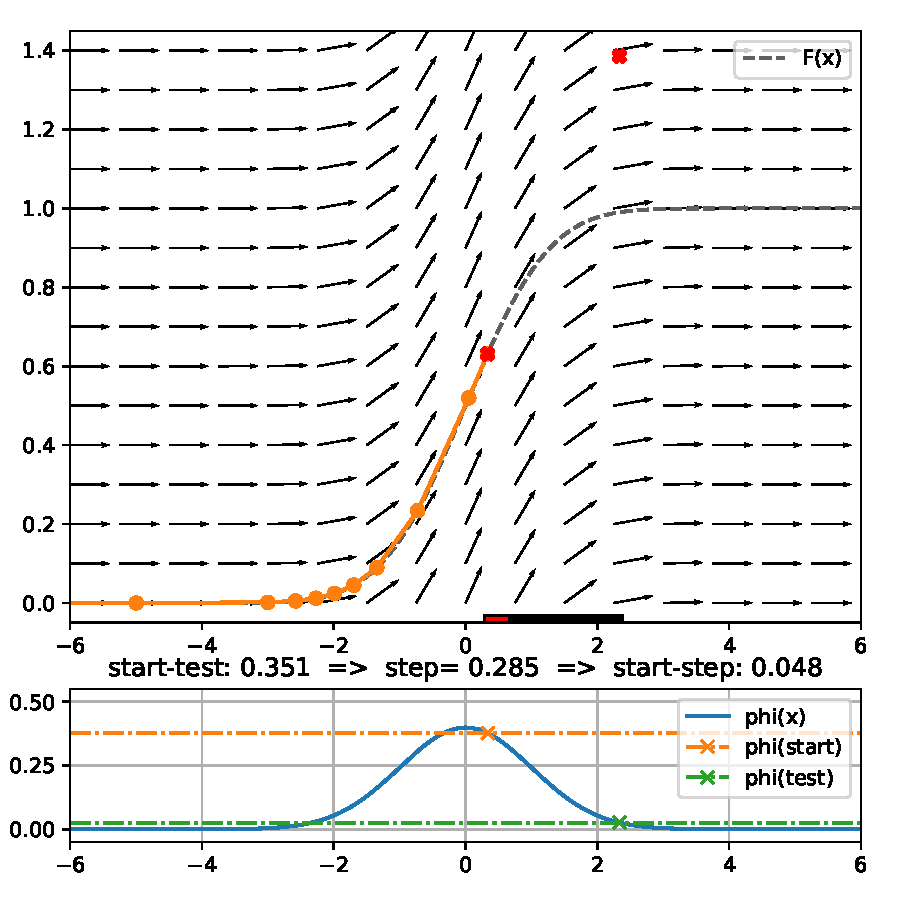
\includegraphics[width=0.5\textwidth]{papers/steps/img/ssc.pdf}
    \caption{Berechnung der Wahrscheinlichkeitsfunktion (oben) der Standardnormalverteilung aus dessen Dichtefunktion (oben mit Pfeilen, unten als Funktion phi(x)) mit einer einfachen Schrittweitensteuerung
      \label{buch:steps:examplessc}}
  \end{figure}

\subsection{Schrittweitensteuerung nach Fehlberg
  \label{steps:subsection:fehlberg}}
Variante nach Fehlberg

\begin{align*}
  k_1 & =f(x_j, u_j)                                                                           \\
  k_2 & =f(x_j + \frac{2}{9}h, u_j+\frac{2}{9}hk_1)                                            \\
  k_3 & =f(x_j + \frac{1}{3}h, u_j+\frac{1}{12}hk_1+\frac{1}{4}hk_2)                           \\
  k_4 & =f(x_j + \frac{3}{4}h, u_j+\frac{69}{128}hk_1-\frac{243}{128}hk_2+\frac{135}{64}hk_3)  \\
  k_5 & =f(x_j + h, u_j-\frac{17}{12}hk_1+\frac{27}{4}hk_2-\frac{27}{5}hk_3+\frac{16}{15}hk_4)
\end{align*}
\[
  u_{j+1} =u_j +h\cdot(\frac{1}{9}k_1+\frac{9}{20}k_3+\frac{16}{45}k_4+\frac{1}{12}k_5)
\]
\[
  k_6 =f(x_j + \frac{5}{6}h, u_j+\frac{65}{432}hk_1-\frac{5}{16}hk_2+\frac{13}{16}hk_3+\frac{4}{27}hk_4+\frac{5}{144}hk_5)
\]
\[
  \hat{u}_{j+1} =u_j+h\cdot(\frac{47}{450}hk_1+\frac{12}{25}hk_3+\frac{32}{225}hk_4+\frac{1}{30}hk_5+\frac{6}{25}hk_6)
\]
\[
  T(x_{j+1},h)=|u_{j+1}-\hat{u}_{j+1}|=\frac{h}{300}\cdot|-2k_1+9k_3-64k_4-15k_5+72k_6|
\]

%\label{steps:embeddedequation}

\begin{figure}
  \centering
  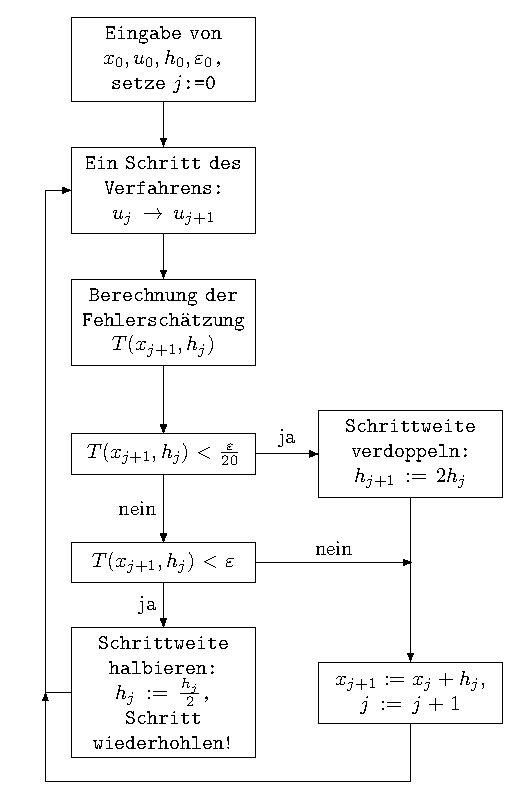
\includegraphics[width=0.5\textwidth]{papers/steps/img/Fehlberg_Flowchart.pdf}
  \caption{Algorithmus zur Schrittlängensteuerung nach Fehlberg
    \label{buch:steps:flowchartfehlberg}}
\end{figure}
